\begin{figure}
	\centering
	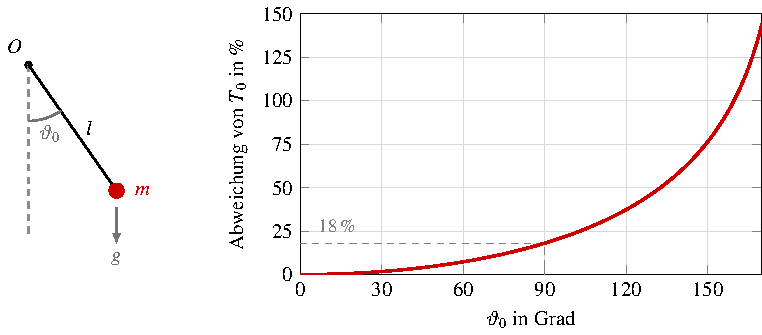
\includegraphics[width=\textwidth]{papers/elliptisch/images/pendel.pdf}
	\caption{Links das mathematische Pendel der Länge $l$ mit der
	Amplitude $\vartheta_0$.
	Rechts die Abweichung der exakten Schwingungsdauer
	$T = 4\sqrt{l/g}\,K(k)$ von der Kleinwinkelnäherung
	$T_0 = 2\pi\sqrt{l/g}$ in Prozent, aufgetragen über
	$\vartheta_0$.
	Bei $90^\circ$ sind es $18\,\%$.}
	\label{fig:elliptisch:pendel}
\end{figure}
